\documentclass[aspectratio=169]{beamer}
%\documentclass[aspectratio=169,handout]{beamer}
\usepackage{pgfpages}
\usepackage[utf8]{inputenc}
\setbeameroption{show notes}
\setbeameroption{show notes on second screen=right}
\usetheme[progressbar=frametitle]{metropolis}

\usepackage[english,german]{babel}
\usepackage[autostyle=true,german=quotes]{csquotes}

% Tikz
\usepackage{tikz}
\usetikzlibrary{arrows,shapes,positioning,shadows,trees,calc}

% Tables
\usepackage{longtable,booktabs}
\usepackage{tabularx}
\usepackage{ltablex}

% Listings
\usepackage{listings}

% Links
\usepackage{hyperref}

% Images
\usepackage{graphicx}

\usepackage{lstlinebgrd}


\title{Projekt Java Compiler}
\subtitle{Spezielle Kapitel der Praktischen Informatik: Compilerbau}
\author{Florian Engel, Robin Heinz, Pavel Karasik, Steffen Lindner, Arwed Mett}
\institute{Universität Tübingen}
\date{05.02.2018}

\begin{document}

	%Titlepage
	\begin{frame}
		\titlepage
	\end{frame}

	%Agenda
	\begin{frame}
		\frametitle{Agenda}
		\tableofcontents
	\end{frame}

	%Chapters
	\section{Allgemein}

\begin{frame}
	\frametitle{Allgemein}
	
\textbf{Aufgabenstellung:}

Entwickeln eines Mini-Java Compilers mit den zugehörigen Schritten: Lexer, Parser, TypChecker und Codegenerierung.
\end{frame}

\begin{frame}[fragile]
\frametitle{Allgemein - Ziel}

\textbf{Ziel} 

Korrektes Übersetzen der folgenden Klasse:

\begin{lstlisting}[language=Java]
class Fibonacci {
  int getFib(int n) {
    return (n < 2) ? n : getFib(n-1) + getFib(n-2);
  }
}
\end{lstlisting}	
\end{frame}



\begin{frame}{Allgemein - Featureliste}

Umgesetze Features (Auszug):

\pause

\begin{itemize}
	\item Ternary Operator \pause
	\item For / While / DoWhile \pause
	\item If / If-Else / Switch-Case \pause 
	\item Pre- bzw. Post Inkrement/Dekrement \pause 
	\item Arithmetische Operatoren (+, -, /, div, mod, *) inklusive Zuweisung (+=, etc.)
\end{itemize}	
\end{frame}

\begin{frame}{Allgemein - Entwicklung}

Code-Sharing über GitHub (https://github.com/Pfeifenjoy/compilerbau-WS17-18) mit continuous integration (travis).

\par \medskip

\pause

Als Build-System wird cabal eingesetzt.	
\end{frame}

\begin{frame}{Allgemein - Projektmanagement}

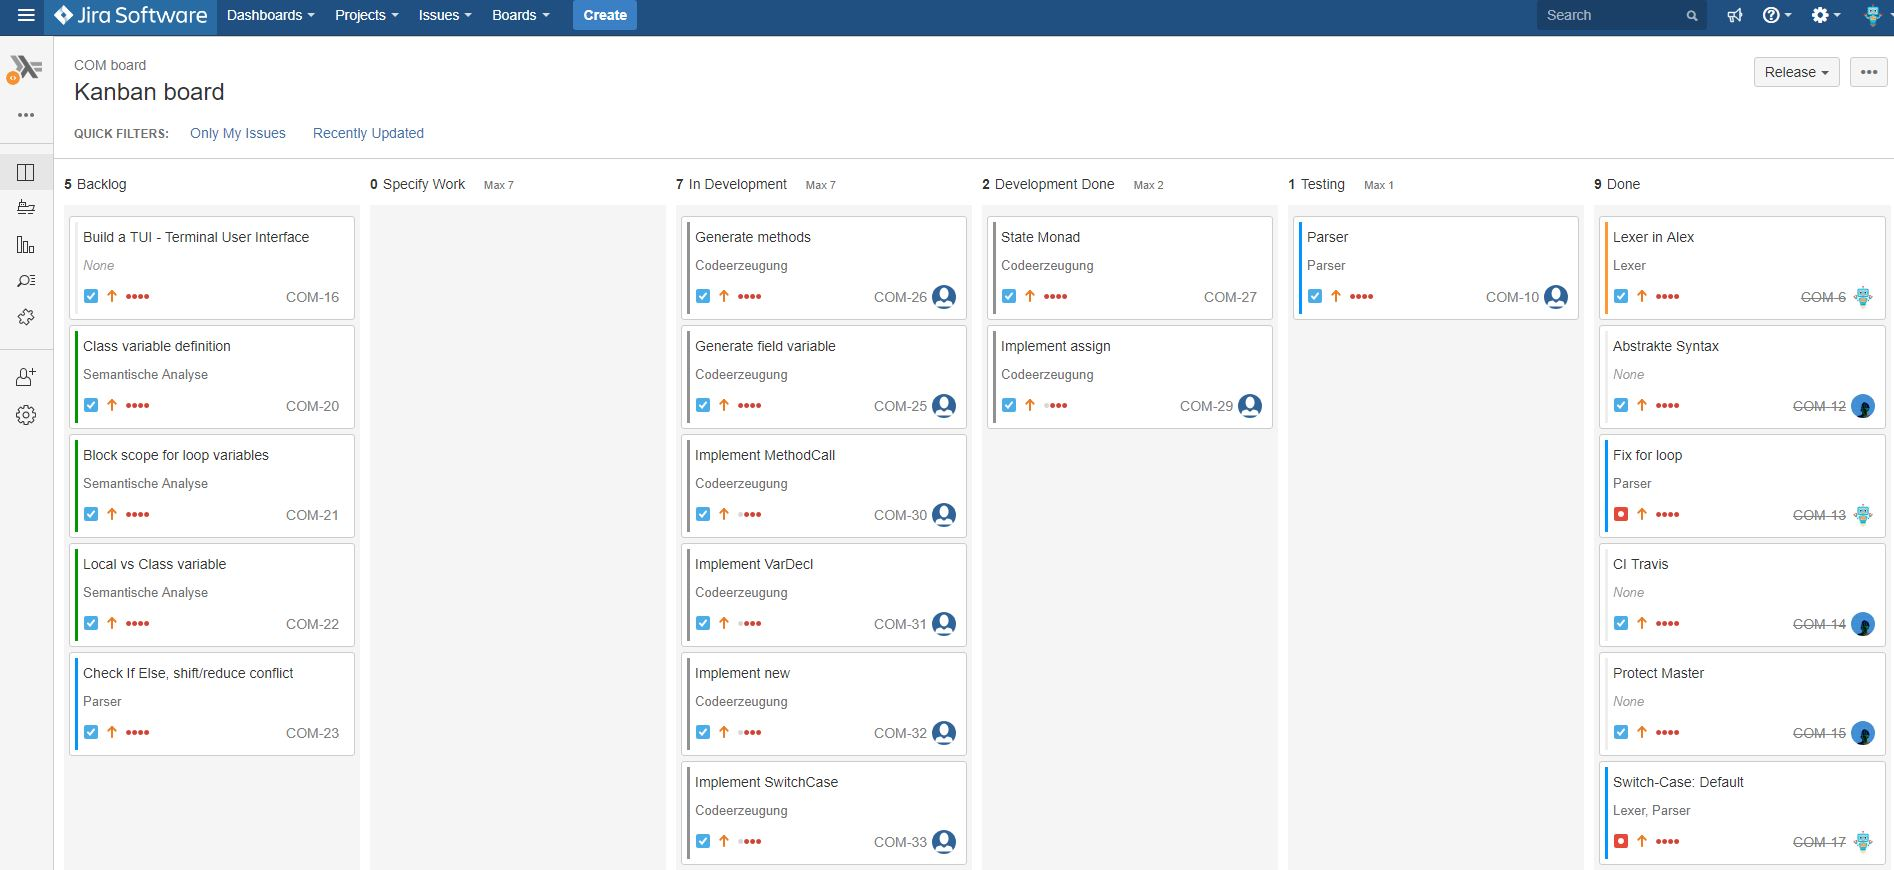
\includegraphics[scale=0.25]{images/allgemein/jira.jpg}

\end{frame}

\begin{frame}{Allgemein - JC}

\begin{itemize}
	\item Text User Interface
	\item Wechseln in Ordner: dist/build/jc
	\item Hilfe: ./jc -h
	\item Compile mit Log: ./jc File.java -l logFile
\end{itemize}

\end{frame}

\begin{frame}{Allgemein - IDE}

\begin{columns}
	\begin{column}{0.5\textwidth}
		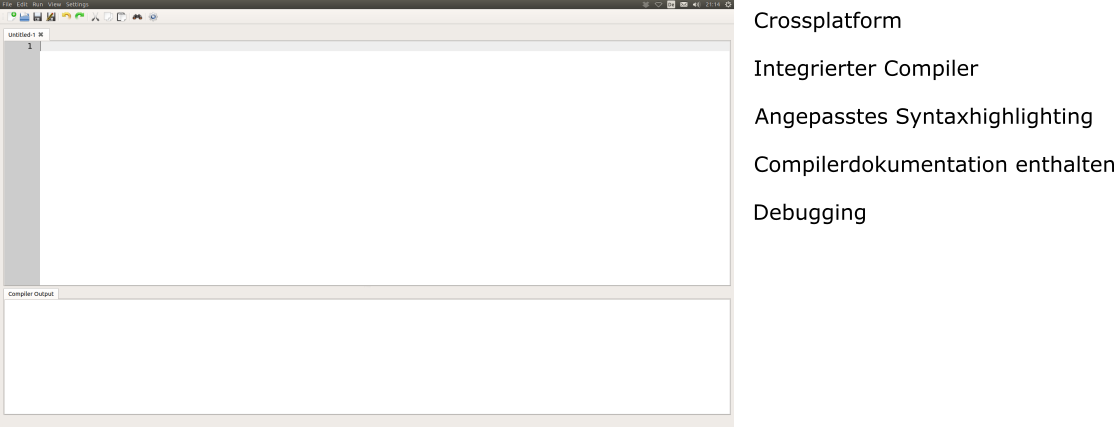
\includegraphics[scale=0.1]{images/allgemein/ide.png}
	\end{column}
	\begin{column}{0.5\textwidth}
			\begin{itemize}
				\item Python: PyQt
				\item Crossplatfrom
				\item Integrierter Compiler
				\item Angepasste Syntaxhighlighting
				\item Compilerdokumentation enthalten
				\item Debugging
			\end{itemize}
	\end{column}
\end{columns}


\end{frame}

	\section{Test-Framework}

\begin{frame}{Test-Framework - Allgemein}
Das Test-Framework wurde selbst implementiert. Es enthält diverse Funktionen zum automatisierten Überprüfen der Testfälle.

\par \medskip

\pause

Tests werden in korrekte und falsche Testfälle unterteilt.


\end{frame}

\begin{frame}[fragile]
	\frametitle{Test-Framework - Token-Coverage \& Testfälle}
	
Die Test-Suite umfasst eine Token-Coverage von 100\%. 

\pause

\par \medskip

Zusätzlich umfasst die Test-Suite insgesamt 21 gültige und 12 ungültige Testfälle.

\pause

\par \medskip

Ungültige Testfälle können in Syntaxfehler (Parser) und Typfehler (Typchecker) eingeteilt werden.
\end{frame}

\begin{frame}{Test-Framework - Testfälle}

Jedes Testfile liegt in einem Ordner (Correct bzw. Wrong) mit zugehöriger .java-Datei. 	

\pause 

\par \medskip

Ein Testfile besteht aus: 

\begin{itemize}
	\item Erwarteten Tokens \pause 
	\item Erwarteter abstrakter Syntax \pause 
	\item Erwarteter getypter abstrakter Syntax \pause
\end{itemize}

Zusätzlich zum eigentlichen Testfile enthält der Ordner ein ClassFile in Haskell, mit der zu erwartenden Struktur des erzeugten Classfiles.
\end{frame}

\begin{frame}[fragile]
\frametitle{Test-Framework - Beispiel Testfile}
\begin{center}
	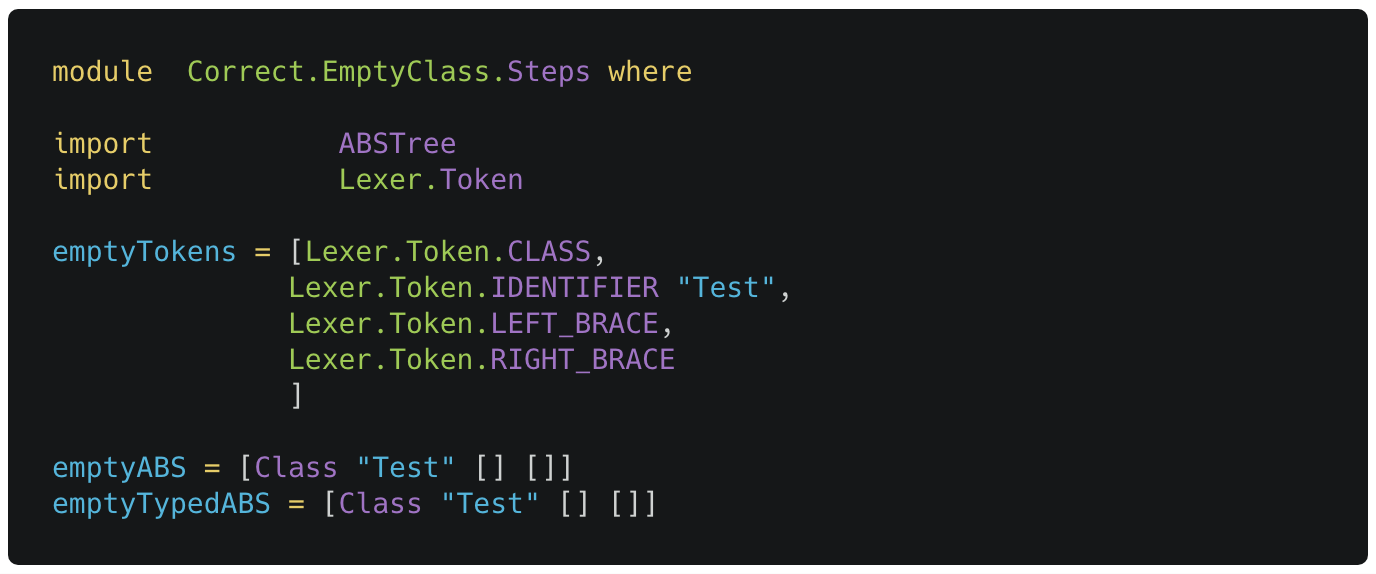
\includegraphics[width=1\textwidth]{images/test-framework/testfile}
\end{center}	
\end{frame}

\begin{frame}{Test-Framework - Beispielprogramme}
Die Testsuite enthält neben den Testfällen auch eine Reihe von (realistischeren) Anwendungsprogrammen. Diese wurden mit 'normalen' Javaprogrammen getestet und werden korrekt compiliert.
\pause

\begin{itemize}
	\item Multiplikation \pause 
	\item Gaußsumme (kleiner Gauß) \pause
	\item Fakultät \pause
	\item Fibonacci \pause
	\item Potenz $a^b$ \pause 
	\item $\lfloor \sqrt{x} \rfloor$ \pause
	\item Primzahltest \& nächste Primzahl ermitteln
\end{itemize}	
\end{frame}

\begin{frame}{Test-Framework: Demo}

	\begin{center}
		\huge{Demo}
	\end{center}
\end{frame}

	\section{Lexer}

\begin{frame}[fragile]
	\frametitle{Tokens}
	\begin{lstlisting}[language=Haskell]
		
data Token
	-- Arithmentics
	= ADD
	| SUBTRACT
	| MULTIPLY
	| DIVIDE
	| MODULO
	| INCREMENT
	| DECREMENT
	-- Logical
	| NOT	
	...	
		
	\end{lstlisting}
\end{frame}

\begin{frame}[fragile]
	\frametitle{Struktur Alex File}
	\begin{lstlisting}[basicstyle=\tiny, language=Haskell]

%wrapper "basic"

$digit = 0-9
$alpha = [a-zA-Z]

tokens :-

	-- Ignore
	$white+ ; 
	"//".*  ;
	
	-- Operators
	-- Arithmetics
	\+                { \s -> ADD }
	\-                { \s -> SUBTRACT }
	\*                { \s -> MULTIPLY }
	\/                { \s -> DIVIDE }	
	...

	\end{lstlisting}
\end{frame}

\begin{frame}{Demo}

\begin{center}
	
\includegraphics{images/lexer/demo.png}
\end{center}

\end{frame}
	\section{Abstrakte Syntax}

\begin{frame}
	\frametitle{Abstrakte Syntax}
	\begin{center}
		\Huge \href{run:../../project/src/ABSTree.hs}{ABSTree.hs}
	\end{center}
\end{frame}

	\section{Parser}

\begin{frame}
	\frametitle{Parser - Allgemein}
	\begin{itemize}
		\item Verwendete Werkzeuge: Happy, Alex
		\item Input: Tokens
		\item Output: ABSTree
		\item Herausforderungen:
			\begin{itemize}
				\item Integration in Build System
				\item Operatoren Priorität
				\item Klassen / Konstruktoren
				\item If-Else
			\end{itemize}
	\end{itemize}
\end{frame}

\begin{frame}[fragile]
	\frametitle{Parser - Integration Build System}
	\begin{lstlisting}[escapechar=!]
library
  exposed-modules:     Lexer, ...
  build-depends:       base <= 4.10.1 ...
  hs-source-dirs:      src
  !\colorbox{yellow}{build-tools:}!            !\colorbox{yellow}{alex, happy}!
  !\colorbox{yellow}{other-modules:}!          !\colorbox{yellow}{Lexer.Lexer, Parser.Parser}!
  default-language:    Haskell2010
	\end{lstlisting}

	\note{
		\begin{itemize}
			\item build-tools
			\item other-modules
		\end{itemize}
	}
\end{frame}

\begin{frame}[fragile]
	\frametitle{Parser - Operatoren Priorität}
	\begin{lstlisting}
%right in                                 //lowest precedence
%right ASSIGN ADD ...
%right QUESTIONMARK COLON
%left OR
...
%nonassoc LESSER GREATER LESSER_EQUAL...
...
%nonassoc INCREMENT DECREMENT             //highest precedence
	\end{lstlisting}
	\note{
		\begin{itemize}
			\item Was ist Operatoren Priorität
			\item Wie wird es in Happy implementiert
			\item Precedence top (low), bottom (high)
			\item Beschreibe Assoziativität
		\end{itemize}
	}
\end{frame}

\begin{frame}[fragile]
	\frametitle{Parser - Struktur Happy File}
	\begin{lstlisting}[basicstyle=\tiny]
		
Program
    : Class                { [$1] }
    | Program Class        { $1 ++ [$2] }
    | Program SEMICOLON    { $1 }

Statement
    : SingleStatement SEMICOLON             { $1 }
	...
    | IF LEFT_PARANTHESES Expression RIGHT_PARANTHESES
        Statement ELSE Statement
                                            { If $3 $5 (Just $7) }
    | IF LEFT_PARANTHESES Expression
        RIGHT_PARANTHESES Statement
        %prec THEN                          { If $3 $5 Nothing }
    | Switch                                { $1 }
	\end{lstlisting}
\end{frame}
\begin{frame}
	\frametitle{Parser - Klassen / Konstruktoren}
	\begin{columns}[T]
	\begin{column}{.48\textwidth}

	\begin{figure}[H]
		\centering
		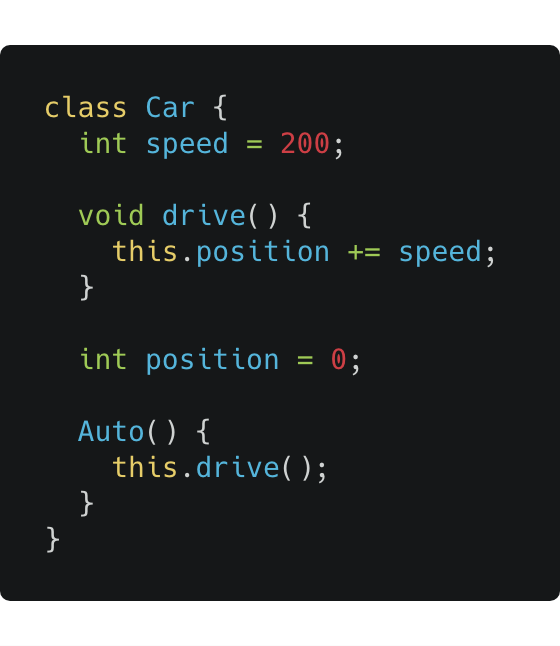
\includegraphics[width=0.6\linewidth]{images/parser/car-class.png}
		\caption{Auto Klasse}
		\label{fig:images/parser/car-class}
	\end{figure}
	\end{column}%
	\hfill%
	\begin{column}{.48\textwidth}

	\pause
	\begin{figure}[H]
		\centering
		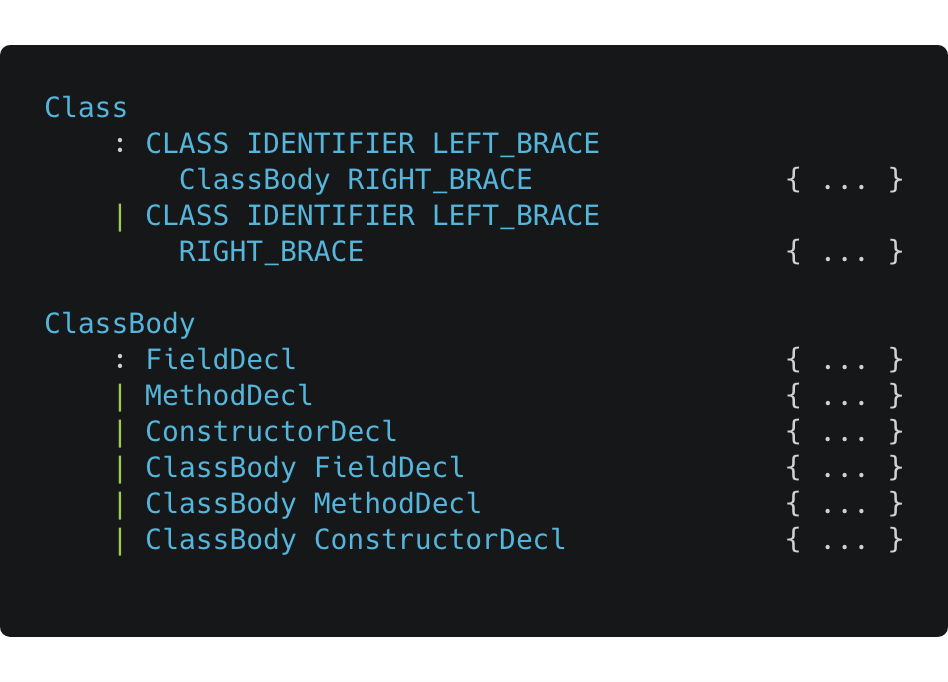
\includegraphics[width=0.95\linewidth]{images/parser/class-ast.png}
		\caption{Grammatik}
		\label{fig:images/parser/class-ast}
	\end{figure}
	\end{column}%
	\end{columns}
\end{frame}

\begin{frame}[fragile]
	\frametitle{Parser - Klassen / Konstruktoren}
	\begin{figure}[H]
		\centering
		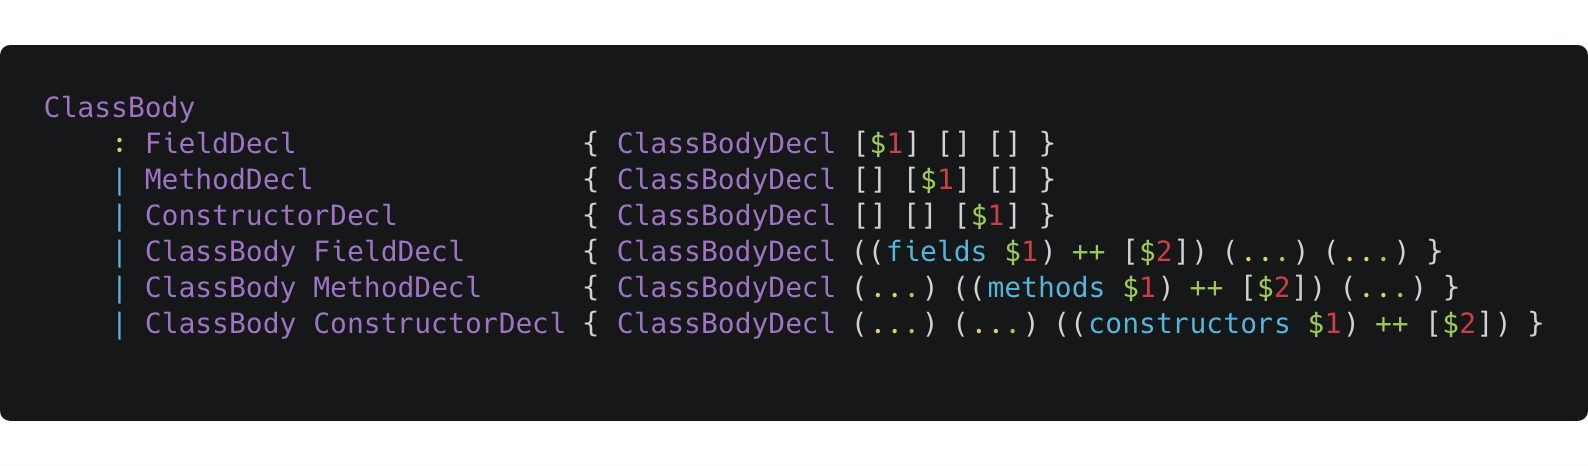
\includegraphics[width=0.9\linewidth]{images/parser/full-class-ast.png}
		\caption{Grammatik - Lösung}
		\label{fig:images/parser/full-class-ast}
	\end{figure}
\end{frame}

\begin{frame}[fragile]
	\frametitle{Parser - If - Else}
	Problem:
	\begin{figure}[H]
		\centering
		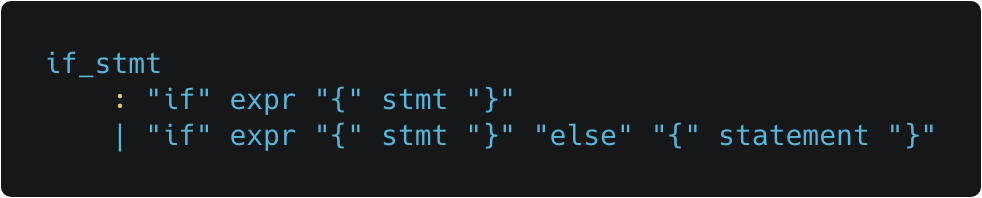
\includegraphics[width=0.7\linewidth]{images/parser/if-else-grammar.png}
	\end{figure}
	\pause
	Solution:

	\begin{figure}[H]
		\centering
		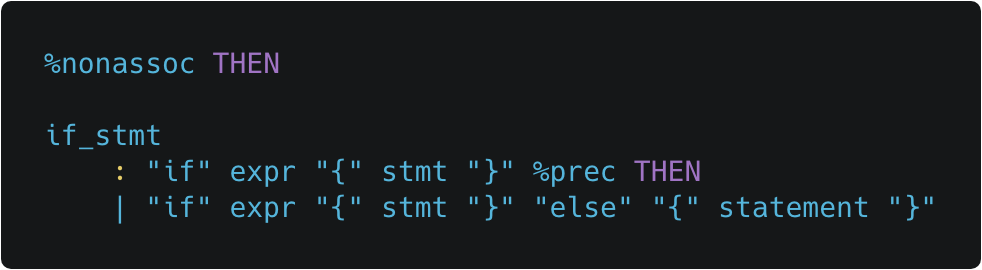
\includegraphics[width=0.7\linewidth]{images/parser/sol-if-else-grammar.png}
	\end{figure}
\end{frame}

\begin{frame}[fragile]
	\frametitle{Beispiel}
	\begin{center}
		\Huge Demo
	\end{center}
\end{frame}


	\section{Typechecker}
\begin{frame}
    \frametitle{Typechecker - Prinzip}

Program liegt als Syntaxbaum (Klassenliste) vor

Der Typechecker:
\begin{itemize}
	\item arbeitetet diesen Baum rekursiv ab (bottom-up)
	\pause
	\item umschließt Expressions/Statements mit Typlabel (string)
	\pause
	\item nutz lookup-Tabellen zur Prüfung der Sichtbarkeit
	\pause
	\item prüft, ob Typen an entsprecheden Stellen zusammenpassen
\end{itemize}
\pause
Typen: int, boolean, char, class-types
\end{frame}

\begin{frame}
    \frametitle{Typechecker - Klassenliste}
${\bf C} = [c_1, \cdots , c_n]$ \\
Iteriere über $C$, für jedes $c \in C$:
\pause
\begin{itemize}
    \item Iteriere über Variablendeklarationen
    \begin{itemize}
        \item Überprüfe Initialdeklarationen der Variablen 
        \item konstruiere (Name:Typ)-Tabelle ${\bf L}$ der Feldvariablen
        \item Klassentyp $"$this$"$
    \end{itemize}
    \pause
    \item Iteriere über Methodendeklarationen
    \begin{itemize}
        \item Prüfe ob Bodytyp (Syntaxbaum) und ReturnTyp zusammenpassen
    \end{itemize}
\end{itemize}
\pause
$\Rightarrow$ Syntaxbaum wird rekursiv abgearbeitet mit ${\bf C}$, ${\bf L}$
\end{frame}

\begin{frame}[fragile]
    \frametitle{Typechecker - Blocks}
Funktionsbody liegt als Block statement (Statemensequenz) vor \\
Returntyp $\rightarrow$ Bodytyp \\
\pause
Handling: fold-Operation wird auf Block ausgeführt
\begin{lstlisting}[language=Haskell]
{ int x = 2; int y = 3; int res = x + y; return res; }	
\end{lstlisting}
\pause
($\{ \}$, void, $L$) \\
\pause
$\Rightarrow$ ($\{"x=2"\}$, void, $L \leftarrow (x,int)$) \\
\pause
$\Rightarrow$ ($\{"x=2","y=3"\}$, void, $L \leftarrow (x,int),(y,int)$) \\
\pause
$\Rightarrow$ ($\{"x=2","y=3","res=x+y"\}$, void, $L \leftarrow (x,int),(y,int),(res,int)$) \\
\pause
$\Rightarrow$ ($\{"x=2","y=3","res=x+y","return"\}$, \bf{int}, $L \leftarrow (x,int),(y,int),(res,int)$) \\
\end{frame}

\begin{frame}
    \frametitle{Typchecker - Expressions (Auszug)}
Klassenliste $C$, Variablenliste $L$ \\
- Literale: True\\
(Booleanliteral True) $\Rightarrow$ ({\bf TypedExpr} (Booleanliteral True) $"$boolean$"$) \\
\pause
- Variablenaufruf: x \\
(LocalOrFieldVar x) \\
$\Rightarrow$ Lookup von x in ${\bf L}$ $\rightarrow$ char \\
$\Rightarrow$ ({\bf TypedExpr} (LocalOrFieldVar x) $"$char$"$) \\
\pause
- Instanzvariablen: x.y \\
(InstVar (x:A) y) \\
$\Rightarrow$ Lookup von A in {\bf C} \\ 
$\Rightarrow$ Lookup von y in A $\rightarrow$ int \\
$\Rightarrow$  ({\bf TypedExpr} (InstVar (x:A) y) $"$int$"$)
 
\end{frame}

\begin{frame}
    \frametitle{Typechecker - Expressionstatements (Auszug)}
Klassenliste $C$, Variablenliste $L$ \\
- Methodenaufruf: x.f(2, 3) \\
(MethodCall (x:A) f (2:int, 3:int)) \\
$\Rightarrow$ Lookup von A in ${\bf C}$ \\
$\Rightarrow$ von f in A $\rightarrow$ returnTyp boolean\\
$\Rightarrow$ Unifikation gegebener und verlangter Argumente \\
$\Rightarrow$ ({\bf TypedStmtExpr} (MethodCall (x:A) f (2:int, 3:int)) $"$boolean$"$) \\
\ \\
\pause
Noch nicht klar, ob als Statement (Typ void) oder als Expression verwendet
\end{frame}

\begin{frame}
    \frametitle{Typechecker - Statements (Auszug)}
Klassenliste $C$, Variablenliste $L$ \\
- Blocks $\{ \cdots \}$\\
Gleiches vorgehen wie bei Funktionsbodys \\
Veränderte Variablenliste $L$ wird verworfen (scope) \\
Bodytype wird auch Bodytype des umgebenden Blocks \\
(Block [$\cdots$]) $\Rightarrow$ ({\bf TypedStmt} (Block [$\cdots$]) blocktype) \\
\ \\
\pause
- Variablendeklarationen: int i = 5;\\
Wie in Felddefinitionen für Klassen \\
${\bf L}$ wird aktualisiert zurückgegeben (shadowing) \\
(LocalVarDecls [$\cdots$]) $\Rightarrow$ ({\bf TypedStmt} (LocalVarDecls [$\cdots$]) $"$void$"$)
\end{frame}
	\section{Code Generator}

\begin{frame}
        \frametitle{Module}
        Die folgenden Module werden für die Erzeugung des Class files aus dem ABSTree benutzt
        \begin{itemize}
                \item genClassFile.hs
                \item genConstantPool.hs
                \item genFields.hs
                \item genMethods.hs
        \end{itemize}
\end{frame}
\begin{frame}
        \frametitle{Module}
        In den nachfolgenden Modulen sind die Datentypen enthalten die für den abstrakten Bytecode benutzt werden
        \begin{itemize}
                \item Data/Assembler.hs
                \item Data/ClassFile.hs
        \end{itemize}
        Aus dem abstrakten Bytecode wird im Module Module BinaryClass.hs der Bytecode erzeugt
\end{frame}
\begin{frame}
        \frametitle{Constanten Pool}
        Der Constantenpool ist in einer hashMap die ein Eintrag auf dessen Position abbildet.

        Im Module genConstantPool.hs sind Funktionen enthalten die ein Eintrag erzeugen und dessen Position zurückgeben bzw nur die Position zurückgeben.
\end{frame}
\begin{frame}[fragile]
        \frametitle{Beispiel genConstantPool}
        \begin{lstlisting}
genMethodRefSuper :: String
                  -> Type
                  -> State ClassFile IndexConstantPool
genMethodRefSuper name typ =
  do indexClassName <- view (super . indexSp) <$> get
     indexNameType <- genNameAndType name typ
     genInfo MethodRefInfo
               { _tagCp              = TagMethodRef
               , _indexNameCp        = indexClassName
               , _indexNameandtypeCp = indexNameType
               , _desc               = ""
               }
        \end{lstlisting}
\end{frame}
\begin{frame}[fragile]
        \frametitle{Generieren der Methoden}
        Bei der Generierung der Methoden werden auch gleichzeitig die Einträge im constanten pool erstellt.  Im State wird folgender Datentyp verwendet.
        \begin{lstlisting}
data Vars
  = Vars { _localVar :: [HM.HashMap LocVarName LocVarIndex]
         , _allLocalVar :: S.Set LocVarName
         , _classFile :: ClassFile
         , _curStack :: Int
         , _maxStack :: Int
         , _line :: LineNumber
         , _continueLine :: [LineNumber]
         }
makeLenses ''Vars
        \end{lstlisting}
\end{frame}

	\section{Fazit}

\begin{frame}{Fazit}

\begin{center}
	
\includegraphics{images/fazit/fazit.png}
\end{center}

\end{frame}

\begin{frame}{Fazit}

\begin{center}
	\begin{tabular}{|c|c|c|c|c|}
		\hline
		Programm & Lexer & Parser & Typchecker & Codegenerator \\
		\hline
		Multiplikation & \checkmark & \checkmark & \checkmark & \checkmark \\
		\hline
		Gaußsumme (kleiner Gauß) & \checkmark & \checkmark & \checkmark & \checkmark \\
		\hline
		\text{Fakultät} & \checkmark & \checkmark & \checkmark & \checkmark \\
		\hline
		Fibonacci & \checkmark & \checkmark & \checkmark & \checkmark \\
		\hline
		Potenz $ a^{b} $ & \checkmark & \checkmark & \checkmark & \checkmark\\
		\hline
	\end{tabular}
\end{center}


\end{frame}
	\begin{frame}[standout]

\flushleft

\textbf{Projekt Java Compiler}

\small{Spezielle Kapitel der Praktischen Informatik: Compilerbau}

Github: \href{https://github.com/Pfeifenjoy/compilerbau-WS17-18}{https://github.com/Pfeifenjoy/compilerbau-WS17-18}

\vspace{1.5cm}

\begin{small}
	Florian Engel, florian.engel@student.uni-tuebingen.de
	
	Robin Heinz, robin.heinz@student.uni-tuebingen.de
	
	Pavel Karasik, pavel.karasik@student.uni-tuebingen.de
	
	Steffen Lindner, steffen.lindner@student.uni-tuebingen.de
	
	Arwed Mett, arwed.mett@student.uni-tuebingen.de
\end{small}
\end{frame}


	% Struktur:
	% Allgemein -> Steffen / Robin
	% - Mit Beispiel anfangen
	% - Beispiel: Multiplikation, Fibonacci
	% - Projektbeschreibung -> Robin
	%   - Start Ende
	%   - Meilensteine
	% - jira -> Robin
	% - Featureliste -> Steffen
	% - travis -> Steffen
	% Test framework -> Steffen
	%  - Aufbau des Frameworks -> Steffen
	%  - Bsp. ein Testfall etc. -> Steffen
	% Lexer -> Robin
	%  - aufbau -> Robin
	% Abstrakte Syntax -> Arwed
	%  - Bsp. zeigen -> Arwed
	%  - Wie sind Typen abgebildet -> Arwed
	% Parser -> Arwed
	%  - Happy File -> Arwed
	%  - Beispiel klasse -> Arwed
	% Typchecker -> Pavel
	%  - Funktionsweise
	%  - Schwierigkeiten
	%  - Lokale Variablen
	%  - nicht sichtbare Variablen
	%  - falsche Rückgabewerte
	% Codegenerierer -> Florian
	%  - Funktionsweise etc.
	%  - Konstantenpool
	% Abschließendes Beispiel -> Florian
	% Fazit -> Robin
	%   - Erfüllt Meilensteine
	% Abschlussfolie
	%  - Namen, mails
	%  - Git repo

\end{document}
